% This is "www2008-sample.tex" copied from "www2005-sample.tex" V1.2 January 26 2004
% This file should be compiled with V1.4 of "www2008-submission.class"
%
% This example file demonstrates the use of the 'www2008-submission.cls'
% V1.4 LaTeX2e document class file. It is for those submitting
% articles to the WWW'04 Conference WHO DO NOT WISH TO 
% STRICTLY ADHERE TO THE SIGS (PUBS-BOARD-ENDORSED) STYLE.
% The 'www2008-submission.cls' file will produce a similar-looking,
% albeit, 'tighter' paper resulting in, invariably, fewer pages.
%
% ----------------------------------------------------------------------------------------------------------------
% This .tex file (and associated .cls V1.4) produces:
%       1) NO Permission Statement
%       2) WWW'04-specific conference (location) information
%       3) The Copyright Line with ACM data
%       4) NO page numbers
%
% ---------------------------------------------------------------------------------------------------------------
% This .tex source is an example which *does* use
% the .bib file (from which the .bbl file % is produced).
% REMEMBER HOWEVER: After having produced the .bbl file,
% and prior to final submission, you *NEED* to 'insert'
% your .bbl file into your source .tex file so as to provide
% ONE 'self-contained' source file.
%
% ================= IF YOU HAVE QUESTIONS =======================
% Questions regarding the SIGS styles, SIGS policies and
% procedures, Conferences etc. should be sent to
% Julie Goetz (goetz@acm.org) or Adrienne Griscti (griscti@acm.org)
%
% Technical questions only to
% Gerald Murray (murray@acm.org)
% ===============================================================
%
% For tracking purposes - this is V1.2 - January 26 2004

\documentclass{../templates/www2008-submission}

% shared affiliation macro
\def\sharedaffiliation{
\end{tabular}
\begin{tabular}{c}}

\begin{document}
%
\title{Bootstrapping the Semantic Web of Social Online Communities}
%\subtitle{[Extended Abstract]
%\titlenote{A full version of this paper is available as
%\textit{Author's Guide to Preparing ACM SIG Proceedings Using
%\LaTeX$2_\epsilon$\ and BibTeX} at
%\texttt{www.acm.org/eaddress.htm}}}
%
% You need the command \numberofauthors to handle the "boxing"
% and alignment of the authors under the title, and to add
% a section for authors number 4 through n.
%
% Up to the first three authors are aligned under the title;
% use the \alignauthor commands below to handle those names
% and affiliations. Add names, affiliations, addresses for
% additional authors as the argument to \additionalauthors;
% these will be set for you without further effort on your
% part as the last section in the body of your article BEFORE
% References or any Appendices.

\numberofauthors{3}
%
% Put no more than the first THREE authors in the \author command

% NOTE: All authors should be on the first page. For instructions
% for more than 3 authors, see:
% http://www.acm.org/sigs/pubs/proceed/sigfaq.htm#a18

%		\author{
%
% The command \alignauthor (no curly braces needed) should
% precede each author name, affiliation/snail-mail address and
% e-mail address. Additionally, tag each line of
% affiliation/address with \affaddr, and tag the
%% e-mail address with \email.

%\alignauthor Diego Berrueta\\
%	\email{diego.berrueta@fundacionctic.org}
%       \affaddr{R\&D Department, Fundaci\'on CTIC}\\
%       \affaddr{Gij\'on, Asturias, Spain}
%\and
%\alignauthor Sergio Fern\'andez\\
%	\email{sergio.fernandez@fundacionctic.org}
%       \affaddr{R\&D Department, Fundaci\'on CTIC}\\
%       \affaddr{Gij\'on, Asturias, Spain}\\
%       \email{\{fname.surname\}@fundacionctic.org}
%\and
%\alignauthor Lian Shi\\
%	\email{lian.shi@fundacionctic.org}
%       \affaddr{R\&D Department, Fundaci\'on CTIC}\\
%       \affaddr{Gij\'on, Asturias, Spain}
%}

\author{
  \alignauthor Diego Berrueta \\
%  \email{diego.berrueta@fundacionctic.org}
%
  \alignauthor Sergio Fern\'andez \\
%  \email{sergio.fernandez@fundacionctic.org}
%
  \alignauthor Lian Shi \\
%  \email{lian.shi@fundacionctic.org}
%
  \sharedaffiliation
    %\email{\{diego.berrueta,sergio.fernandez,lian.shi\}@fundacionctic.org}
    \affaddr{\texttt{\{diego.berrueta,sergio.fernandez,lian.shi\}@fundacionctic.org}} \\
    \affaddr{R\&D Department, Fundaci\'on CTIC}  \\
    \affaddr{Gij\'on, Asturias, Spain}
}

%\additionalauthors{Additional authors: John Smith (The Th{\o}rv\"{a}ld Group,
%email: {\texttt{jsmith@affiliation.org}}) and Julius P.~Kumquat
%(The Kumquat Consortium, email: {\texttt{jpkumquat@consortium.net}}).}

%\date{5 February 2008}

\maketitle

\begin{abstract}
Mining and searching the social web is hardly possible without
a noteworthy amount of data available in an interoperable
format. This paper enumerates and compares several techniques which can be
applied to obtain large quantities of RDF data describing
social web sites. Advantages, drawbacks and potential issues of
each of these methods are discussed. Practical experimentation
permits to illustrate and to discuss the convenience of each approach.
\end{abstract}

% A category with only the three required fields
%\category{E.0}{Data}{General}
\category{M.0}{Knowledge Management}{Knowledge Acquisition}
\category{M.7}{Knowledge Management}{Knowledge Retrieval}

\keywords{semantic mining, online community, mailing list, rdf, xsl, foaf, sioc, semantic web, social web}

%%%%%%%%%%%%%%%%%%%%%%%%%%%%%%%%%%%%%%%%%%%%%%%%%%%%%%%%%%%%
\section{Introduction}

Effective large-scale mining of the social web requires the
availability of big amounts of well-defined data~\cite{Mika2004}.
The semantic web provides a convenient platform to publish and
consume this data. There are a couple of semantic web vocabularies
which are particularly suited to represent the
information of the social web using an interoperable formalism.
However, currently only a small portion of the social web is
represented in these vocabularies.

In this paper we survey and classify a number of methods that
are targeted to create semantic web enabled representations of
the information of the social web. We focus on online communities
and discussion forums, although the methods described here are also valid
for other social web sites. The combination of all of them
may provide enough momentum to the semantic social
web and it can help to reach the critical-mass that
enables a virtuous cycle of applications and data.

The rest of the paper is organized as follows: in Section~\ref{sec:vocabularies}
the FOAF and SIOC vocabularies are introduced in the context of applying
the semantic web to the description of the social web. Section~\ref{sec:taxonomy}
enumerates and classifies some methods to produce large quantities
of RDF descriptions. Section~\ref{sec:case-studies} and
Section~\ref{sec:experimentation} address two paradigmatic methods
and their experimental application. Some issues which appear
frequently are described in Section~\ref{sec:problems}, and
finally Section~\ref{sec:conclusions} discusses the future of the
semantic social web and concludes the paper.


%%%%%%%%%%%%%%%%%%%%%%%%%%%%%%%%%%%%%%%%%%%%%%%%%%%%%%%%%%%%
\section{Semantic Web Vocabularies to describe the Social Web}\label{sec:vocabularies}

The Semantic Web initiative uses RDF (Resource Description
Framework~\cite{RDF}) as the (meta)data representation model.
Ontologies are artifacts that define the meaning of the symbols
which appear in the RDF assertions. Two ontologies are
specially relevant to describe the social web: FOAF and SIOC.

FOAF~\cite{FOAF} is one of the most used vocabularies in the documents that
constitute the current Semantic Web~\cite{Ding2005, Finin2005}.
It provides the essential classes and properties necessary
to describe individuals
and their relationships. However, FOAF descriptions can be found
only for a very small portion of the web users. Bootstrapping the
FOAF-web by means of mining the document-web is the topic
of~\cite{Mika2004}. Consequently, the focus of our work is not the
description of people. Instead, this paper focuses on the description
of the interactions between people in online discussion communities.

DERI NUI Galway leads the development of SIOC (Seman\-ti\-cally-Interlinked Online
Communities\footnote{\texttt{http://sioc-project.org/}}), an ontology which 
defines a vocabulary to interconnect different discussion methods such 
as blogs, web-based forums and mailing lists~\cite{Breslin2006,Breslin2005}.
SIOC is now an official W3C member submission~\cite{Bojars2007}.
SIOC provides the foundations to describe online discussion
communities using RDF (users, forums and posts), as illustrated in
Figure~\ref{fig:sioc}.

\begin{figure}
 \centering
 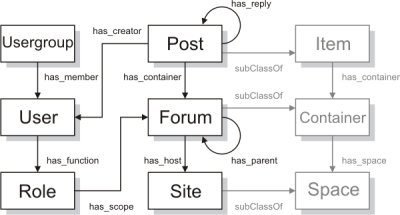
\includegraphics[width=8cm]{images/sioc.png}
 \caption{\label{fig:sioc}SIOC main classes and properties, reproduced from the SIOC specification.}
\end{figure}

In the rest of the paper, we describe methods to create a large
quantity of RDF instances of the SIOC ontology.


%%%%%%%%%%%%%%%%%%%%%%%%%%%%%%%%%%%%%%%%%%%%%%%%%%%%%%%%%%%%
\section{Methods to Mass-produce SIOC Instances}\label{sec:taxonomy}

Since SIOC is a recent specification, its adoption is still low, and
only a few sites export SIOC data. There exist a number of techniques
that can be used to bootstrap a network of semantic descriptions from
current social web sites. We classify them in two main categories:

\begin{itemize}
\item On the one hand, methods which require direct access to the underlying database behind
the social web site are \emph{intrusive techniques}.
\item On the other hand, methods which do not require direct access to
the database and can operate on resources already published on the web
are \emph{non-intrusive}.
\end{itemize}

We further describe each kind in the following paragraphs.

\subsection{Intrusive techniques}

It is safe to say that every social web site is built on top of a
database that serves as its information model. The web application
acts as the controller and publishes different views of the model in
formats such as HTML and RSS. In terms of this pattern, publishing
SIOC data is as simple as adding a new view.
From a functional point of view, this is the most powerful scenario, because
it allows a lossless publication due to the direct access
to the back-end database.

The SIOC community has contributed a number of plug-ins for some
popular web community-building applications, such as Drupal, WordPress and 
PhpBB\footnote{A more complete and up-to-date list is available
at \texttt{http://sioc-project.org/exporters}.}. Mailing lists are
also covered by SWAML, which is described later in this paper.

There is, however, a major blocker for this approach. All these
software components need a deployment in the server side (where
the database is). This is a burden for system administrators, who
are often unwilling to make a move that would make it more difficult to
maintain, keep secure and upgrade their systems. This is particularly
true when there is no obvious immediate benefit of exporting
SIOC data (\emph{chicken-and-egg} problem).

\subsection{Unintrusive techniques}

In absence of direct access to the database, unintrusive
techniques exploit the information already available on the web:

\begin{itemize}

\item Cooked HTML views of the information, the same ones that
are rendered by web browsers for human consumption. Even if this 
source is always available, its exploitation poses a number of 
issues described in Section~\ref{sec:problems}.

\item RSS/Atom feeds, which have become very popular in the recent years.
They can be easily
translated into SIOC instances using XSLT stylesheets (for XML-based feeds) or 
SPARQL queries\footnote{\texttt{http://tinyurl.com/2u3e6k}} (for RSS 1.0, 
which is actually RDF). Unfortunately, these feeds often contain just 
partial descriptions.

\item Public APIs. The Web~2.0 trend has pushed some social web
sites to export (part of) their functionality through APIs
in order to enable their consumption by third-party mash-ups and applications.
Where available, these APIs offer an excellent opportunity to
create RDF views of the data.

\end{itemize}

A shared aspect of these sources is their ubiquitous availability through
web protocols and languages, such as HTTP and XML. Therefore, they
can be consumed anywhere, and thus system administrators are freed of
taking care of any additional deployment. In contrast, they cannot compete
with the intrusive approaches in terms of information quality, as
their access to the data is not primary.

% TODO
% But with this approach is necessary to know the issues with sites not
% permitting non-intrusive access )terms of service, robots.txt, etc).

%%%%%%%%%%%%%%%%%%%%%%%%%%%%%%%%%%%%%%%%%%%%%%%%%%%%%%%%%%%%
\section{Case studies}\label{sec:case-studies}

In this section we describe an example of each of the two approaches
aforementioned.

\subsection{From mboxes to RDF: SWAML}

SWAML~\cite{SWAML2007} is a Python script that reads mailing 
list archives in raw format, typically stored in a ``mailbox'' 
(or ``mbox''), as defined in RFC~4155~\cite{RFC4155}. It parses
mailboxes and outputs RDF descriptions of the messages, mailing lists
and users as instances of the SIOC ontology. Internally, it re-constructs
the structure of the conversations in a tree structure, and it exploits
this structure to produce links between the posts.

This script is highly configurable and non-interactive, and has been
designed to be invoked by the system task scheduler. This low-coupling with
the software that runs the mailing list eases its portability and
deployment.

SWAML classifies as an intrusive technique because
it requires access to the primary data source, even if in this case
it is not a relational database but a text file. Anyway, it is
worth mentioning that some servers publish these text files
(mailboxes) through HTTP. Therefore, sometimes it is possible to
retrieve the mailbox and build a perfect replica of the primary
database in another box. In such cases, SWAML can be used without the
participation of the system administration of the original
web server.

\subsection{HTML Scraping with XSLT}

Web scraping is a well-known, non-intrusive and widely used technique,
although it should be applied only when other approaches are not viable.
Screen-scraping applications are difficult to maintain and
often produce low-quality information.

A popular language to write HTML scrapers is XSLT. As a prerequisite,
the mark-up must be converted to XHTML (an XML dialect) if it is not
already in this format. Fortunately, open source utilities such as
Tidy\footnote{\texttt{http://tidy.sourceforge.net/}} do a decent job
to clean and fix HTML files with a poor mark-up.

Scraping functions are often tied to a web crawler to follow the
links between HTML pages.

As each web site uses a different, customized template to
publish their cooked HTML files, it is
difficult to develop a generic scraper, even for a single social
web application. Moreover, there are lots of different social and
web community-building applications, and thus the portability of scrapers
is very low.

The output of a web scraper implemented in XSLT is usually RDF/XML, but
another interesting possibility has already been explored. In
mle~\cite{Hausenblas2007}, the authors use XSLT to decorate the
DOM tree of an XHTML page with RDFa attributes~\cite{Birbeck2006}.
This creates an hybrid representation which is readable for
humans \emph{and} semantic web agents.


%%%%%%%%%%%%%%%%%%%%%%%%%%%%%%%%%%%%%%%%%%%%%%%%%%%%%%%%%%%%
\section{Experimentation}\label{sec:experimentation}

Some experiments were run following the case studies described above.
We chose the Free Software communities as the target of our
experimentation because they are characterized for their openness and
they offer a huge number of very popular online discussion forums.
Among those, we picked two clusters: the GNOME project mailing lists and
the Debian mailing lists. Although both of them contain the same
kind of forum (mailing lists), they are tackled with different methods,
as explained below. The result, anyway, is the same in both cases:
a big dataset of RDF instances that can be uploaded to an RDF
store such as Sesame~\cite{Broekstra2002}. In this way, they can be
queried and mined. Moreover, it is also possible to execute rules or
inference engines to obtain new knowledge.

\subsection{GNOME mailing lists}\label{sec:gnome}

GNOME is a graphical desktop environment available as free
software. It has a vibrant community of users and developers
who communicate over the Internet using IRC and mailing lists.
The web site of the GNOME project publishes the complete archive
of near 200 mailing lists during the ten year of activity of
the project\footnote{\texttt{http://mail.gnome.org/archives/}}.
These archives are published not just as cooked HTML files for
human consumption, but also as gzipped mailboxes split by
month and mailing list.

A simple shell script was run to fetch, unpack and concatenate the
mailboxes into a single file for each mailing list. These files
were provided as input data to SWAML. The
result was a dataset that contains more than 25 million RDF triples.

\subsection{Debian mailing lists}\label{sec:debian}

Debian is a compilation of free software that constitutes a
complete operating system~\cite{Krafft2005}. It is the result of a
collaborative effort by a thousand developers since 1993, and it has
millions of users (as often happens with open source software, it is very
difficult to estimate the actual number of users). Together, developers
and users constitute a very active community, and they use the web and
mailing lists as communication channels. Some of the 180 official mailing
lists have almost 30,000~members and up to
7,000~messages/month\footnote{Information collected from \texttt{http://lists.debian.org/stats/}, Feb 10, 2008.}.

The mailboxes of these mailing lists are not available on the web, but
the complete archive of the messages is published as a set of
HTML files generated by MHonArc. We crawled a subset of these files
(11 mailing lists in the period 2005-2006) and collected almost 220,000
messages. The mark-up of each file was fixed and converted to XHTML Strict
using Tidy. Finally, an XSLT stylesheet was applied to produce a
RDF description for each message. In order to simplify the
task of translating dates to a uniform ISO format, we extended
the Xalan XSLT processor with custom functions implemented in Java.

The resulting dataset sums up more that 3 million RDF triples. The
memory space required to store this dataset can be notably
reduced if the body of the messages is dropped, i.e., if only the meta-data
is kept. We envision that many mining applications will not need the
body of the messages.

%\subsection{\label{sec:ubuntu}Ubuntu Forums}
%
%Ubuntu Forums\footnote{\texttt{http://ubuntuforums.org/}} are a very popular 
%discussion forums among users of this GNU/Linux distribution. They have a 
%frenetic activity, with plus than 4 million of posts in the moment we made
%our experiments.
%
%In these forums we used a quite similar appoach than with Debian mailing
%lists. We analized the markup generated by vBulletin (CMS used in these forums)
%and we developed some XSLT stylesheets to transform get instances of
%\texttt{sioc:Forum}, \texttt{sioc:Thread} and \texttt{sioc:Post}. We 
%selected only a subset of available forums to test our application,
%although the results have been quite poor because the informaion and 
%markup aren't very well organized.


%%%%%%%%%%%%%%%%%%%%%%%%%%%%%%%%%%%%%%%%%%%%%%%%%%%%%%%%%%%%
\section{Common issues}\label{sec:problems}

When put into practice, some shared problems and limitations
of the approaches described above are revealed:

\begin{itemize}
  \item \emph{Same person, multiple identities}. A single individual can
        participate in several social web sites, often under a different
        virtual identity. Over the years, this individual can own a
        number of user accounts and e-mail addresses, which are modelled
        as different entities in SIOC. If each of these were taken as
        a different person, social web mining would lead to imprecise
        conclusions.

        FOAF separates the description of a person
        (\texttt{Person})
        from the description of her user accounts (\texttt{OnlineAccount}).
        This makes it possible to establish one-to-many relationships
        between these entities, see Figure~\ref{fig:foaf-sioc}.

	\begin{figure}[t]
	 \centering
	 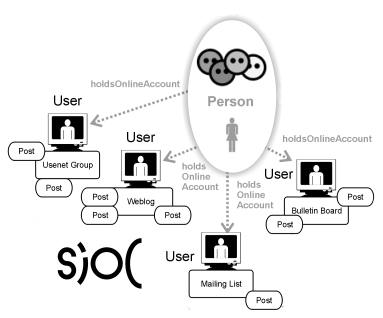
\includegraphics[width=8cm]{images/foaf-sioc.png}
	 \caption{\label{fig:foaf-sioc}Relationship between FOAF and SIOC. Image by John Breslin, reproduced from \texttt{http://sioc-project.org/node/158}.}
	\end{figure}

        From the perspective of an automatic processing of the
        information, the challenge is to build these links. In an
        ideal scenario, the FOAF description of an individual would
        contain such links. In practice, these links must be
        inferred from coincident values of some properties such
        as the e-mail address or the URL of the personal home page.
        In the worst case, the only way to go is to perform heuristic matching
        using the person's name or nickname.

        A comprehensive knowledge base of FOAF descriptions can prove
        very useful in this task. However, it introduces another related issue:
        as anyone can create FOAF descriptions, there may exist more than
        one instance of \texttt{foaf:Person} in the knowledge base
        to describe the same person.
        Consolidation of these instances is a similar problem to the
        one just described, and receives the name of "instance
        smushing"\footnote{\texttt{http://esw.w3.org/topic/RdfSmushing}}.
        For our experiments, we crawled a dataset 4,000 FOAF descriptions
        from Advogato\footnote{\texttt{http://www.advogato.org/}}, a social
        network for free software developers.

  \item \emph{Hashed e-mail addresses}. Both FOAF and SIOC
        rely on the sha1 algorithm~\cite{Eastlake2001} to represent
        e-mail addresses in an opaque way. The main purpose to do so
        is to block spammers, who otherwise would find it easy to collect
        e-mail addresses. It is
        assumed that hashed e-mail addresses retain their capability
        as unique identifiers of the resources. However, neither
        the FOAF nor the SIOC specification describe a normalization
        procedure to be applied to the e-mail address, besides adding
        the \texttt{mailto:} prefix. This is unfortunate, because it
        fails to prevent equivalent
        e-mail addresses from producing different hashed values. For instance,
        it is common to find spelling variants of the same
        e-mail address which only differ on the use of lower and upper-case
        letters. These variants produce irreconcilable values
        when the hash function is applied, thus making them unusable
        to spot equivalent instances of the same resource.

  \item \emph{Flat threads}. Typically, web-based discussion forums and blogs
        have flat threads, i.e., all the replies are attached to the original
        post that started the thread. However, discussions hosted in those
        forums often violate this restrictive pattern, and some messages
        are in fact replies to some of the precedent ones. Users often
        quote the actual message they are replying to in order to clarify the
        flow. Unfortunately, it is difficult to automatically re-build
        the actual hierarchical structure of the conversation. Therefore,
        when converted to SIOC, some information about the sequence of
        the discussion is lost.

        The situation is completely different for mailing lists, because
        each new post contains a header (\texttt{In-Reply-To}) that points
        to the immediate parent in the thread hierarchy.

  \item \emph{Repeated primary keys}. Every online discussion community assigns
        an identifier (primary key) to each message and user. These
        identifiers are locally unique, and can be used to coin a URI
        for each resource. Mailing lists also use identifiers
        (\texttt{Message-ID}, as defined in RFC~2822~\cite{RFC2822}) for
        each e-mail message, although in this case, such identifiers are
        supposed to be globally-unique. However, non RFC-compliant or
        improperly configured mail transport agents can potentially produce repeated
        identifiers for e-mail messages. Our experimentation has
        revealed that it is possible to find clashes among the messages
        of a mailing list. This fact leads to two consequences. Firstly,
        \texttt{Message-ID}s cannot be used to coin URIs. Secondly,
        links between messages, such as those created by the
        \texttt{In-Reply-To} header, are not fully reliable.

  \item \emph{Pagination}. Long discussions and indexes are often paginated
        into several inter-linked HTML files. Although web crawlers can
        retrieve all parts, this fragmentation poses a challenge for
        scraping the information. It is often necessary to re-join the
        different pages in order to produce a consistent RDF representation
        of the information.

\end{itemize}


%%%%%%%%%%%%%%%%%%%%%%%%%%%%%%%%%%%%%%%%%%%%%%%%%%%%%%%%%%%%
\section{Conclusions}\label{sec:conclusions}

Machine-readable descriptions of online communities enable them
to be mined in a more efficient way. So far, the availability of
such descriptions has been low. The semantic web provides the
best framework to publish and consume formalized descriptions of
the artifacts that are part of the social web. In this paper,
we presented some state-of-the-art techniques which can be
put into practice to instantiate the social semantic web.

Each scenario dictates different requisites, and thus, a different
technique. The intrusive ones are clearly preferred due to their
closeness to the primary source (the database), but sometimes they may be
unpractical because of deployment issues.

In the long term, we foresee that FOAF and SIOC-enabling plug-ins
will become commodities in the software that supports the social
web. The RSS is the most immediate precedent of a similar semantic web
technology which has permeated into the mainstream web. These information-rich
descriptions will
be available for both machines and humans by means of HTTP
content negotiation~\cite{Recipes} or hybrid representations (RDFa).


% The following two commands are all you need in the
% initial runs of your .tex file to
% produce the bibliography for the citations in your paper.
\bibliographystyle{abbrv}
\bibliography{../references}

\balancecolumns

\end{document}
